\documentclass[a4paper,12pt]{jarticle}
\usepackage[dvipdfmx]{graphicx}
\usepackage[dvipdfmx]{color}
\usepackage{tabularx}
\topmargin=10mm

\title{物理学実験1 課題}
\author{B6SB2006  石川祐也}
\date{2017/11/21}

\begin{document}

\section{目的}

\section{課題1}

\newpage

\section{課題2 吸収係数の測定(石川)}
 \subsection{原理}
 \subsubsection{吸収係数}
 $\gamma$線は通過するとき、相互作用を起こしながら一個一個ビーム束から失われていく。
 通過前に$I_0$個の$\gamma$線が厚さ$x$の物を通過すると、通過後の$\gamma$線の個数$I$は、
 $$I(x)=I_0 \exp^{-\mu x}$$
 となる。$\mu$は$\gamma$線が単位暑さを通る間に失われる確率を表した量であり、全吸収係数と呼ばれる。
 これは光電効果、コンプトン効果、電子対生成効果の相互作用によって決まる。

 \subsubsection{解析}
 課題1の解析方法に準じる。

 \subsection{実験方法}
  \subsubsection{試料・装置}
   実験試料
   \begin{itemize}
    \item $^{60}$Co線源
    \item $^{137}$Cs線源
    \item 吸収体Al
    \item 吸収体Pb
   \end{itemize}

   実験装置
    \begin{itemize}
     \item ノギス
     \item コリメータ
     \item 検出器
     \item 吸収体固定器具
    \end{itemize}

  \subsubsection{手順}
   \begin{enumerate}
    \item 吸収体2種類各4枚の暑さをノギスで測定した。
    \item 検出器、吸収体固定器具、コリメータ、線源の順に配置した。
    \item 吸収体それぞれにおいて、枚数を4,3,2,1,0枚と変化させながら300秒間測定した。
    \item Co線源より1.33,1.17MeV,Cs線源より0.662MeVにおける2種類の吸収体の質量吸収係数を求めた。
   \end{enumerate}


 \subsection{結果}
  測定結果を表\ref{table:Cs137}〜表\ref{table:Co60_right}、
  図\ref{fig:Cs137}〜図\ref{fig:Co60_right}に示す。
  \begin{table}[htbp]
   \begin{center}

       \caption{Cs線源(0.662MeV)におけるカウント数}
        \begin{tabular}{|r|r|r|r|}
         \hline
         条件 & thickness$[g/cm^2]$ & counts & count-err \\
         \hline
         \hline
         Pb*4 & 91.37  & 407.883  & 10.729  \\
         Pb*3 & 67.53  & 516.345  & 11.460  \\
         Pb*2 & 44.83  & 628.302  & 12.794  \\
         Pb*1 & 22.98  & 791.932  & 16.199  \\
         Pb*0 & 0.00  & 975.312  & 19.112  \\
         \hline
         Al*4 & 4.394  & 713.589  & 16.030  \\
         Al*3 & 3.294  & 779.481  & 15.410  \\
         Al*2 & 2.194  & 800.105  & 15.871  \\
         Al*1 & 1.094  & 865.602  & 16.667  \\
         Al*0 & 0.000  & 916.487  & 18.576  \\
         \hline
        \end{tabular}
       \label{table:Cs137}

   \end{center}
  \end{table}

  \begin{table}[htbp]
   \begin{center}

       \caption{Co線源(1.17MeV)におけるカウント数}
        \begin{tabular}{|r|r|r|r|}
         \hline
         条件 & thickness$[g/cm^2]$ & counts & count-err \\
         \hline
         \hline
         Pb*4 & 91.37  & 377.318  & 16.044  \\
         Pb*3 & 67.53  & 480.421  & 18.995  \\
         Pb*2 & 44.83  & 494.764  & 17.330  \\
         Pb*1 & 22.98  & 605.956  & 21.885  \\
         Pb*0 & 0.00  & 695.440  & 20.696  \\
        \hline
        Al*4 & 4.394  & 588.768  & 20.998  \\
        Al*3 & 3.294  & 585.289  & 20.783  \\
        Al*2 & 2.194  & 649.388  & 21.835  \\
        Al*1 & 1.094  & 676.884  & 22.603  \\
        Al*0 & 0.000  & 710.113  & 20.801  \\
         \hline
        \end{tabular}
       \label{table:Co60_left}

   \end{center}
  \end{table}


  \begin{table}[htbp]
   \begin{center}

       \caption{Co線源(1.33MeV)におけるカウント数}
        \begin{tabular}{|r|r|r|r|}
         \hline
         条件 & thickness$[g/cm^2]$ & counts & count-err \\
         \hline
         \hline
         Pb*4 & 91.37  & 368.798  & 18.781  \\
         Pb*3 & 67.53  & 474.963  & 21.952  \\
         Pb*2 & 44.83  & 468.756  & 21.003  \\
         Pb*1 & 22.98  & 572.481  & 25.054  \\
         Pb*0 & 0.00  & 637.676  & 23.621  \\
         \hline
         Al*4 & 4.394  & 530.308  & 25.082  \\
         Al*3 & 3.294  & 542.671  & 25.208  \\
         Al*2 & 2.194  & 606.691  & 25.864  \\
         Al*1 & 1.094  & 636.237  & 27.067  \\
         Al*0 & 0.000  & 637.661  & 24.523  \\

         \hline
        \end{tabular}
       \label{table:Co60_right}

   \end{center}
  \end{table}

  \begin{figure}[htbp]
   \begin{center}
   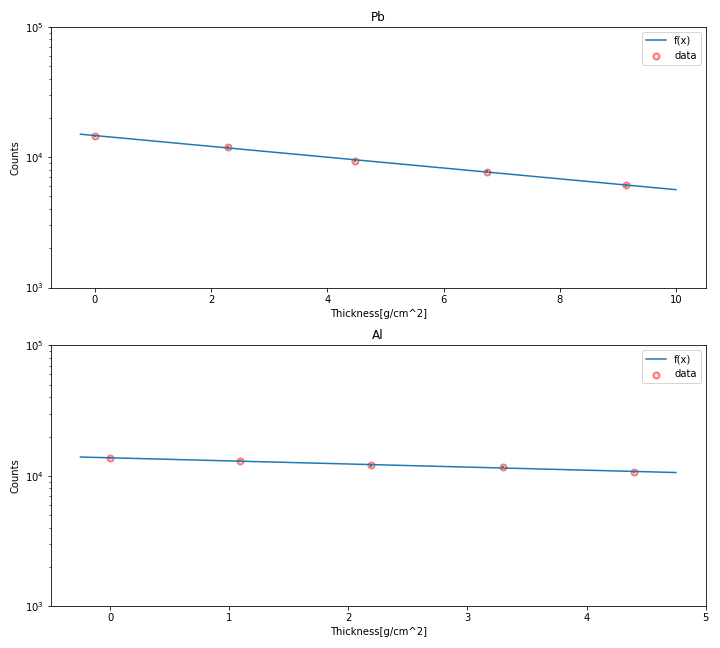
\includegraphics[clip,width=14.0cm]{Cs137.png}
    \caption{0.662MeV(Cs137)における各吸収体の厚さとカウント数}
    \label{fig:Cs137}
   \end{center}
  \end{figure}

  \begin{figure}[htbp]
   \begin{center}
   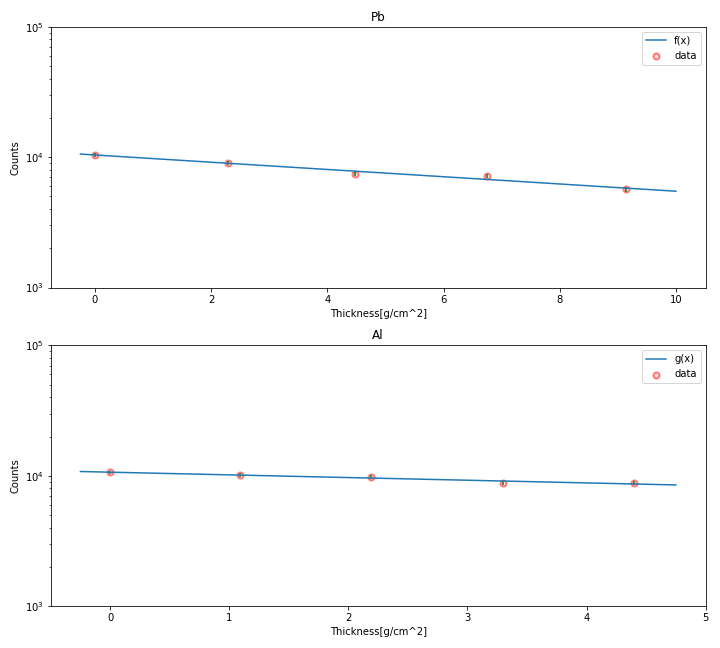
\includegraphics[clip,width=14.0cm]{Co60_left.png}
    \caption{1.17MeV(Co60)における各吸収体の厚さとカウント数}
    \label{fig:Co60_left}
   \end{center}
  \end{figure}

  \begin{figure}[htbp]
   \begin{center}
   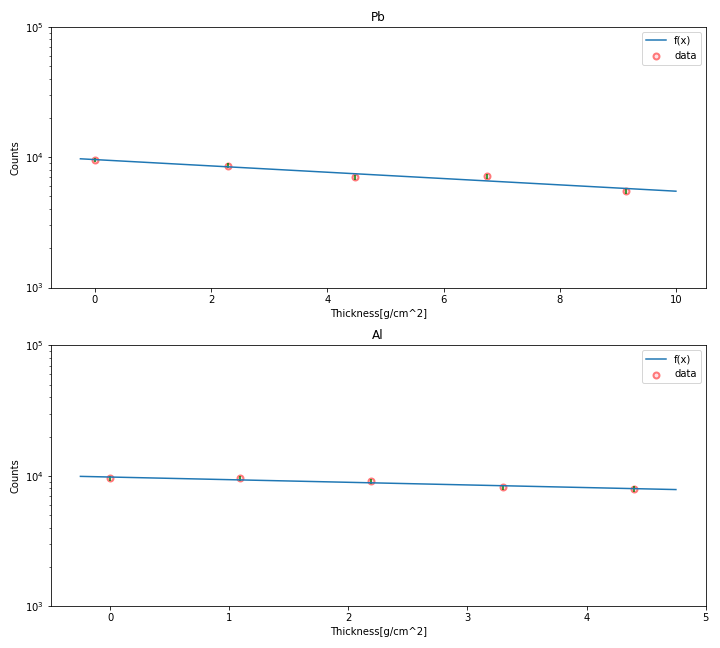
\includegraphics[clip,width=14.0cm]{Co60_right.png}
    \caption{1.33MeV(Co60)における各吸収体の厚さとカウント数}
    \label{fig:Co60_right}
   \end{center}
  \end{figure}


  \begin{table}[h]
   \begin{center}

       \caption{エネルギーと各吸収体における吸収係数}
        \begin{tabular}{|r|r|r|r|r|}
         \hline
         吸収体 & energy[MeV] & $\mu[cm^-1]$ & 誤差 & reduced-chisquare \\
         \hline
         Pb & 0.662  & 0.096  & 0.003  & 0.252  \\
         Pb & 1.173  & 0.064  & 0.005  & 1.749  \\
         Pb & 1.332  & 0.056  & 0.006  & 1.857  \\
         Al & 0.662  & 0.055  & 0.006  & 0.566  \\
         Al & 1.173  & 0.047  & 0.009  & 0.546  \\
         Al & 1.332  & 0.047  & 0.012  & 0.548  \\
         \hline
        \end{tabular}
       \label{table:result}

   \end{center}
  \end{table}

  \begin{figure}[htbp]
   \begin{center}
   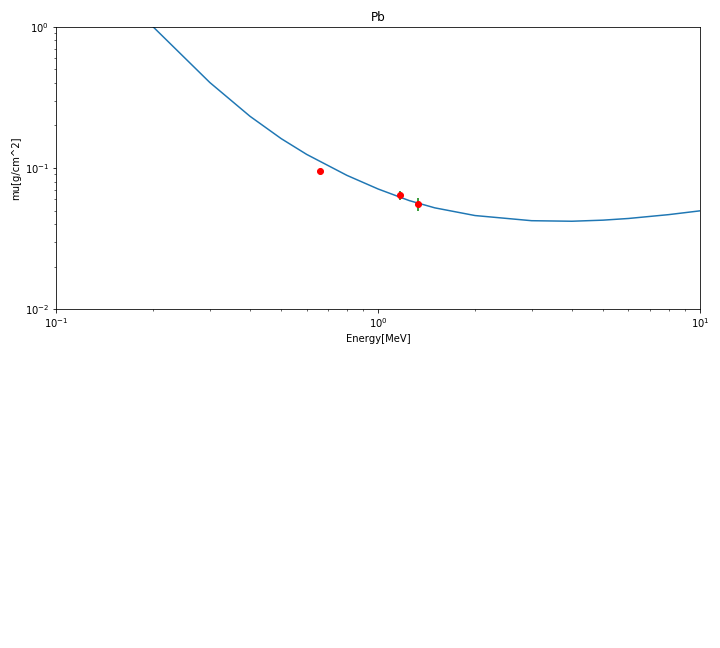
\includegraphics[clip,width=14.0cm]{result_Pb.png}
    \caption{Pbにおける吸収係数の文献値と測定値の比較}
    \label{fig:result_Pb}
   \end{center}
  \end{figure}

  \begin{figure}[htbp]
   \begin{center}
   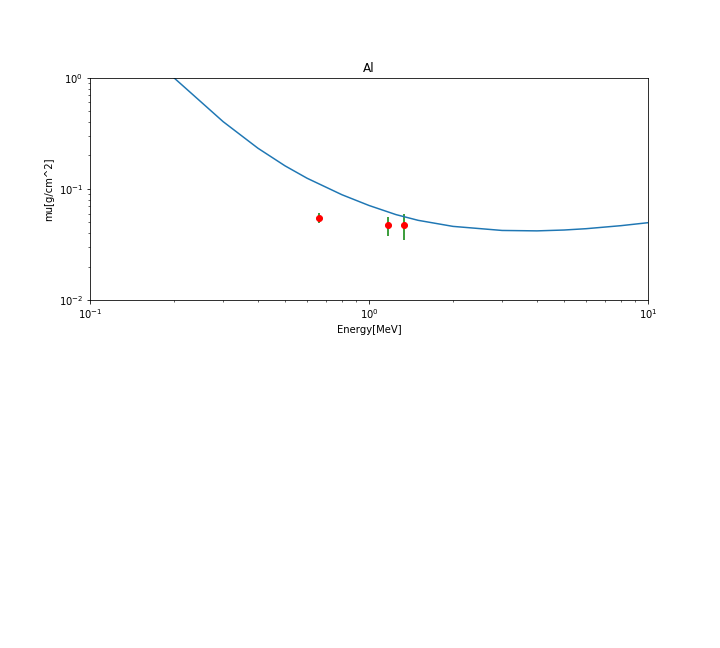
\includegraphics[clip,width=14.0cm]{result_Al.png}
    \caption{Alにおける吸収係数の文献値と測定値の比較}
    \label{fig:result_Al}
   \end{center}
  \end{figure}



 \subsection{考察}
 測定結果と文献値の比較すると、測定結果は概ね文献値に一致している事が伺える。
 しかし完全に一致しているとは言い難い。
 これは、吸収体の厚さの測定誤差が影響していると考えられる。また表\ref{table:result}より換算カイ二乗の
 値を読み取ると、フィッティングの精度がやや低い事が伺える。ゆえにフィッティングを用いて推定した
 カウントの値の正確性が低く、吸収係数の推定の精度が低くなったと考えられる。


\section{実験3 不安定核の崩壊の測定(石川)}
 \subsection{原理}
  \subsubsection{半減期}
原子核等の崩壊過程は始状態と終状態とその崩壊を起こす相互作用によって決定される。
初めにに$N_0$個のアイソトープがあったとすると、時間tが経過した後のアイソトープの個数$N$は、
$$N(t)=N_0 \exp^{-\lambda t}$$
となる。$\lambda$は「寿命$\tau$」の逆数で表される量である。また半減期$T_0$とは、
$N=\frac{N_0}{2}$になるまでかかる時間であり、
$$T_0 = \frac{\ln 2}{T_0}$$
の関係がある。

  \subsubsection{解析}
  課題1の解析方法に準じる。

 \subsection{実験方法}
  \subsubsection{試料・装置}
   実験試料
   \begin{itemize}
    \item $^{198}$Au
   \end{itemize}

   実験装置
    \begin{itemize}
     \item コリメータ
     \item 検出器
     \item サンプルホルダ
    \end{itemize}

  \subsubsection{手順}
   \begin{enumerate}
    \item サイクロトロンセンターで金サンプルビームの照射を行い不安定核である
    $^{198}Au$サンプルを作成した。
    \item 検出器、吸収体固定器具、コリメータ、線源の順に配置した。
    \item 一定時間経過ごとに900秒間測定した。
    \item 測定結果より$^{198}Au$の半減期を求めた。
   \end{enumerate}

 \subsection{結果}
  測定結果を表\ref{table:3r}、図\ref{fig:Au}に示す。
  \begin{table}[htbp]
   \begin{center}

       \caption{測定時間とエネルギーピーク}
        \begin{tabular}{|r|r|r|}
         \hline
         測定時刻   &  エネルギー[MeV] & err \\
         \hline
         2018/6/6/16:21  & 0.425265 & 0.006  \\
         2018/6/7/13:19  & 0.425021 & 0.006  \\
         2018/6/13/13:20 & 0.427356 & 0.004  \\
         2018/6/14/13:20 & 0.428244 & 0.006  \\
         \hline
        \end{tabular}
       \label{table:3r}

   \end{center}
  \end{table}


  \begin{figure}[htbp]
   \begin{center}
   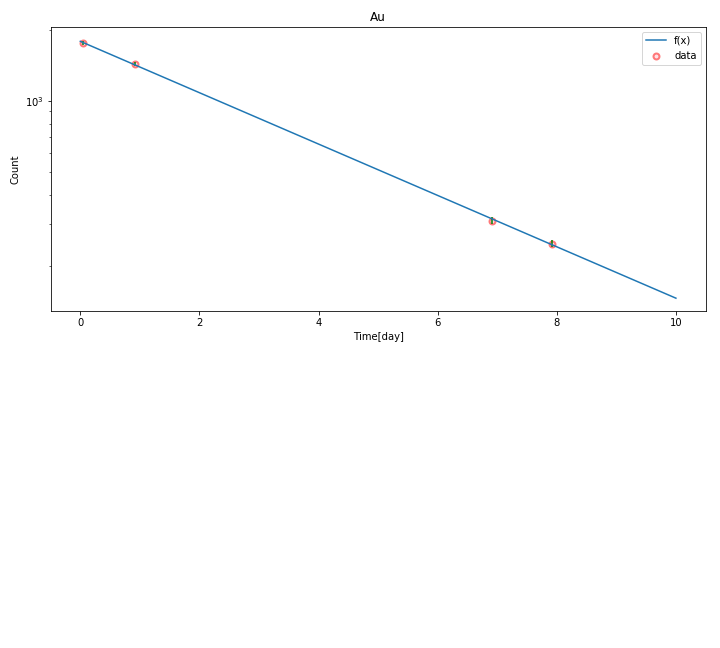
\includegraphics[clip,width=14.0cm]{Au.png}
    \caption{Au}
    \label{fig:Au}
   \end{center}
  \end{figure}

 \subsection{考察}
 表\ref{table:3r}と文献値0.41180[MeV]と比較すると、文献値が誤差の範囲内に収まっていないことが分かる。
 これは課題1で述べたが、較正曲線が厳密には1次関数でフィッテングできない為であると考えられる。\\
 また半減期$T_0$ は $2.77 \pm 0.04$[日]と求められた。これは2$\sigma$の範囲に文献値2.696[日]が収まる。
 誤差の原因としては、表\ref{table:3r}においてエネルギーピークの位置が変化しているように見えることから、一定として
 考えていた印加電圧がずれてしまっていることが考えられる。また電源をつけてすぐに測定を行なっていた実験
 があった為、光電子増倍菅の電源電圧が安定していなかったことが影響していると考えられる。

 \section{結論}
 各種測定を行うことで、$\gamma$線の測定原理について理解を深めることが出来た。また測定結果の考察を通して
 測定の際に気をつけるべき手順について学ぶことができた。



\end{document}
